% Title: gl2ps_renderer figure
% Creator: GL2PS 1.4.0, (C) 1999-2017 C. Geuzaine
% For: Octave
% CreationDate: Fri Dec 29 11:40:15 2017
\setlength{\unitlength}{1pt}
\begin{picture}(0,0)
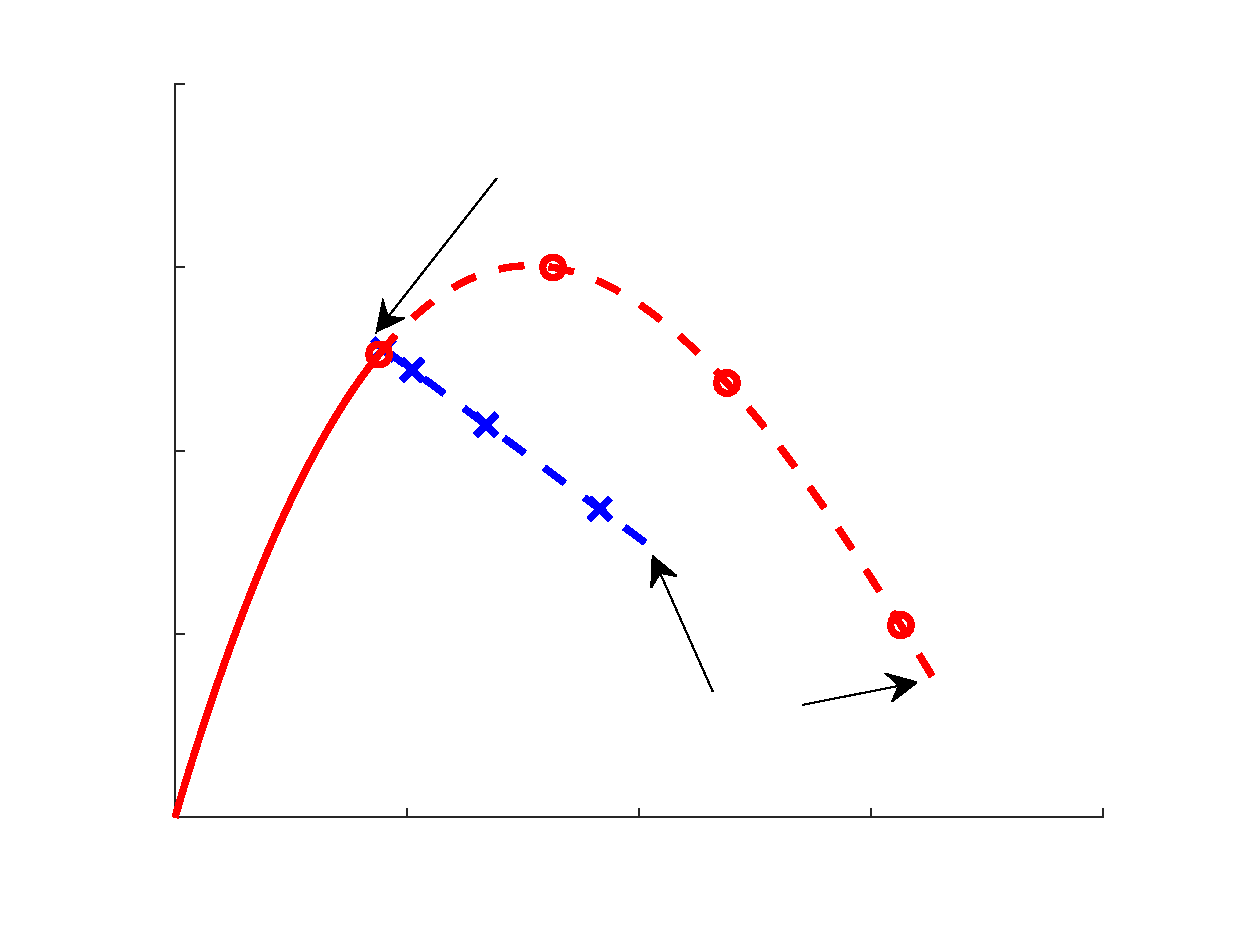
\includegraphics{figli-inc}
\end{picture}%
\begin{picture}(576,432)(0,0)
\fontsize{15}{0}
\selectfont\put(76.0013,42.5189){\makebox(0,0)[t]{\textcolor[rgb]{0.15,0.15,0.15}{{0}}}}
\fontsize{15}{0}
\selectfont\put(187.321,42.5189){\makebox(0,0)[t]{\textcolor[rgb]{0.15,0.15,0.15}{{50}}}}
\fontsize{15}{0}
\selectfont\put(298.641,42.5189){\makebox(0,0)[t]{\textcolor[rgb]{0.15,0.15,0.15}{{100}}}}
\fontsize{15}{0}
\selectfont\put(409.96,42.5189){\makebox(0,0)[t]{\textcolor[rgb]{0.15,0.15,0.15}{{150}}}}
\fontsize{15}{0}
\selectfont\put(521.28,42.5189){\makebox(0,0)[t]{\textcolor[rgb]{0.15,0.15,0.15}{{200}}}}
\fontsize{15}{0}
\selectfont\put(70.9981,47.52){\makebox(0,0)[r]{\textcolor[rgb]{0.15,0.15,0.15}{{0}}}}
\fontsize{15}{0}
\selectfont\put(70.9981,135.54){\makebox(0,0)[r]{\textcolor[rgb]{0.15,0.15,0.15}{{5000}}}}
\fontsize{15}{0}
\selectfont\put(70.9981,223.56){\makebox(0,0)[r]{\textcolor[rgb]{0.15,0.15,0.15}{{10000}}}}
\fontsize{15}{0}
\selectfont\put(70.9981,311.58){\makebox(0,0)[r]{\textcolor[rgb]{0.15,0.15,0.15}{{15000}}}}
\fontsize{15}{0}
\selectfont\put(70.9981,399.6){\makebox(0,0)[r]{\textcolor[rgb]{0.15,0.15,0.15}{{20000}}}}
\fontsize{14}{0}
\selectfont\put(298.641,24.5188){\makebox(0,0)[t]{\textcolor[rgb]{0.15,0.15,0.15}{{Desplazamiento vertical (cm)}}}}
\fontsize{14}{0}
\selectfont\put(16.9981,223.56){\rotatebox{90}{\makebox(0,0)[b]{\textcolor[rgb]{0.15,0.15,0.15}{{Fuerza aplicada (kN)}}}}}
\fontsize{15}{0}
\selectfont\put(275.08,100){\makebox(0,0)[l]{\textcolor[rgb]{0,0,0}{{Ramas inestables}}}}
\fontsize{15}{0}
\selectfont\put(230.4,362.24){\makebox(0,0)[l]{\textcolor[rgb]{0,0,0}{{Punto de bifuraci\'on}}}}
\end{picture}
